%%%%%%%%%%%%%%%%%%%%%%%%%%%%%%%%%%%%%%%%%%%%%%%%%%%%%%%%%%%%%%%%%%%%%%%%%%%
%
% Generic template for TFC/TFM/TFG/Tesis
%
% $Id: resultados.tex,v 1.2 2013/12/12 23:06:55 macias Exp $
%
% By:
%  + Javier Mac�as-Guarasa. 
%    Departamento de Electr�nica
%    Universidad de Alcal�
%  + Roberto Barra-Chicote. 
%    Departamento de Ingenier�a Electr�nica
%    Universidad Polit�cnica de Madrid   
% 
% Based on original sources by Roberto Barra, Manuel Oca�a, Jes�s Nuevo,
% Pedro Revenga, Fernando Herr�nz and Noelia Hern�ndez. Thanks a lot to
% all of them, and to the many anonymous contributors found (thanks to
% google) that provided help in setting all this up.
%
% See also the additionalContributors.txt file to check the name of
% additional contributors to this work.
%
% If you think you can add pieces of relevant/useful examples,
% improvements, please contact us at (macias@depeca.uah.es)
%
% Copyleft 2013
%
%%%%%%%%%%%%%%%%%%%%%%%%%%%%%%%%%%%%%%%%%%%%%%%%%%%%%%%%%%%%%%%%%%%%%%%%%%%

\chapter{Resultados}
\label{cha:resultados}


\begin{FraseCelebre}
  \begin{Frase}
    % Si quieres ser le�do m�s de una vez, no vaciles en borrar a menudo.
    Rem tene, verba sequentur (Si dominas el tema, las palabras vendr�n
    solas)\footnote{Tomado de ejemplos del proyecto \texis{}.}.
  \end{Frase}
  \begin{Fuente}
    % Horacio
    Cat�n el Viejo
  \end{Fuente}
\end{FraseCelebre}

\section{Introducci�n}
\label{sec:introduccion-resultados}

En este cap�tulo se introducir�n los resultados m�s relevantes del
trabajo. 

La estructura del cap�tulo es\ldots


\section{Entorno experimental}
\label{sec:entorno-experimental}

Blah, blah, blah.


\subsection{Bases de datos utilizadas}
\label{sec:bases-de-datos-1}

Blah, blah, blah.


\subsection{M�tricas de calidad}
\label{sec:metricas-de-calidad}

Blah, blah, blah.


\subsection{Estrategia y metodolog�a de experimentaci�n}
\label{sec:estr-y-metod}

Blah, blah, blah.


\section{Resultados experimentales}
\label{sec:result-experim}

A continuaci�n, se muestra un ejemplo de tabla simple (ver tabla \ref{table1}).

\begin{table}
  % increase table row spacing, adjust to taste
  \renewcommand{\arraystretch}{1.3}
  \caption{Comparativa.}
  \label{table1}
  \begin{center}
    % Some packages, such as MDW tools, offer better commands for making tables
    % than the plain LaTeX2e tabular which is used here.
    \begin{tabular}{|c|c|c|}
      \hline
      Method & Training Time & Man-Work (\%)\\
      \hline
      Propagation model & $<$ 30 sec & 5\\
      \hline
      Manual & 9 h 30 min & 24\\
      \hline
      Automatic & 2 h & 10 8\\
      \hline
    \end{tabular}
  \end{center}
\end{table}

Cuando las tablas ocupan m�s de un p�gina se debe utilizar un tipo
especial de tablas denominado \texttt{longtable}. A continuaci�n, se
muestra un ejemplo del mismo (ver tabla \ref{table2}).

\begin{center}
	\begin{longtable}{|c|c|c|c|}
    \caption[Resultados de la correlaci�n cruzada.]{Resultados de la correlaci�n cruzada.} \label{table2} \\
    
    \hline \multicolumn{1}{|c|}{\textbf{Posici�n Real}} & \multicolumn{1}{c|}{\textbf{Posici�n estimada}} & \multicolumn{1}{c|}{\textbf{Coef. Correlaci�n}} & \multicolumn{1}{c|}{\textbf{Acierto/Fallo}} \\ \hline 
    \endfirsthead
    
    \multicolumn{4}{c}%
    {{\bfseries \tablename\ \thetable{} -- contin�a en la p�gina anterior}} \\
    \hline \multicolumn{1}{|c|}{\textbf{Posici�n Real}} & \multicolumn{1}{c|}{\textbf{Posici�n estimada}} & \multicolumn{1}{c|}{\textbf{Coef. Correlaci�n}} & \multicolumn{1}{c|}{\textbf{Acierto/Fallo}} \\ \hline 
    \endhead
    
    \hline \multicolumn{4}{|r|}{{Contin�a en la p�gina siguiente}} \\ \hline
    \endfoot

    \hline \hline
    \endlastfoot
    
    \hline	2P0	&	2P0	&	0,004954	&	A	\\
    \hline	2P1	&	2P4	&	0,005752	&	F	\\
    \hline	2P2	&	2P2	&	0,005461	&	A	\\
    \hline	2P3	&	2P0	&	0,004634	&	F	\\
    \hline	2P5	&	2P4	&	0,005991	&	F	\\
    \hline	2P6	&	2P16	&	0,004410	&	F	\\
    \hline	2P7	&	3P9	&	0,008038	&	F	\\
    \hline	2P8	&	3P9	&	0,003753	&	F	\\
    \hline	2P9	&	2P7	&	0,004908	&	F	\\
    \hline	2P10	&	2P10	&	0,007273	&	A	\\
    \hline	2P14	&	2P16	&	0,006485	&	F	\\
    \hline	2P15	&	2P15	&	0,004932	&	A	\\
    \hline	2P16	&	2P16	&	0,006237	&	A	\\
    \hline	2P17	&	2P15	&	0,005110	&	F	\\
    \hline	2P18	&	3P18	&	0,006235	&	F	\\
    \hline	2P19	&	3P18	&	0,004827	&	F	\\
    \hline	2P20	&	2P20	&	0,006877	&	A	\\
    \hline	2P22	&	3P18	&	0,003048	&	F	\\
    \hline	2P24	&	2P24	&	0,006833	&	A	\\
    \hline	2P25	&	2P25	&	0,004875	&	A	\\
    \hline	2P26	&	2P31	&	0,005511	&	F	\\
    \hline	2P27	&	2P28	&	0,004590	&	F	\\
    \hline	2P30	&	2P31	&	0,005576	&	F	\\
    \hline	2P31	&	2P31	&	0,007213	&	A	\\
    \hline	2P32	&	2P35	&	0,003340	&	F	\\
    \hline	2P34	&	2P34	&	0,004128	&	A	\\
    \hline	2P36	&	2P35	&	0,003329	&	F	\\
    \hline	2P37	&	2P37	&	0,003468	&	A	\\
    \hline	2P39	&	2P38	&	0,002577	&	F	\\
    \hline	2P40	&	2P43	&	0,004303	&	F	\\
    \hline	2P41	&	2P41	&	0,001573	&	A	\\
    \hline	2P42	&	2P41	&	0,000846	&	F	\\
    \hline	2P44	&	2P44	&	0,002732	&	A	\\
    \hline	2P45	&	23P45	&	0,001958	&	F	\\
    \hline	2P47	&	2P34	&	0,002869	&	F	\\
    \hline	2P48	&	2P43	&	0,004569	&	F	\\
    \hline	2P49	&	3P51	&	0,001374	&	F	\\
    \hline	2P50	&	2P34	&	0,002274	&	F	\\
    \hline	2P51	&	2P63	&	0,003931	&	F	\\
    \hline	2P52	&	2P55	&	0,003537	&	F	\\
    \hline	2P53	&	3P56	&	0,003126	&	F	\\
    \hline	2P54	&	2P67	&	0,005560	&	F	\\
    \hline	2P56	&	2P55	&	0,002817	&	F	\\
    \hline	2P57	&	2P67	&	0,006168	&	F	\\
    \hline	2P58	&	2P58	&	0,005278	&	A	\\
    \hline	2P60	&	3P66	&	0,004966	&	F	\\
    \hline	2P61	&	3P61	&	0,004748	&	A	\\
    \hline	2P64	&	2P67	&	0,005342	&	F	\\
    \hline	2P66	&	2P4	&	0,004172	&	F	\\
    \hline	2P67	&	2P67	&	0,005706	&	A	\\
    \hline	3P0	&	3P0	&	0,003674	&	A	\\
    \hline	3P61	&	2P61	&	0,003263	&	F	\\
    \hline	3P64	&	2P67	&	0,003484	&	F	\\
    \hline	3P65	&	2P67	&	0,002975	&	F	\\
    \hline	3P66	&	2P58	&	0,005029	&	F	\\
    \hline	3P67	&	3P67	&	0,003714	&	A	\\
	\end{longtable}
\end{center}

En algunas ocasiones, tambi�n resulta �til emplear el entorno
\texttt{subfloat} (del paquete \texttt{subfig}) para a�adir m�ltiples
im�genes dentro de la misma figura. A continuaci�n, se muestra un
ejemplo del uso en la figura \ref{fig:fig2}. Tambi�n se pueden
referenciar las sub-figuras de forma individual, por ejemplo la
sub-figura \ref{fig:fig2b} (usando un m�todo de cita), o bien la
sub-figura \ref{fig:fig2}\subref{fig:fig2b} (usando otro alternativo).

\begin{figure}[h]
  \centerline{\subfloat[Mean entropy]{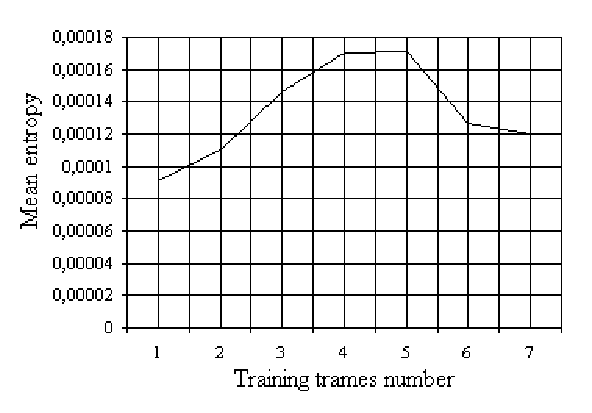
\includegraphics[width=3in]{Figure2}
      % where an .eps filename suffix will be assumed under latex, 
      % and a .pdf suffix will be assumed for pdflatex
      \label{fig:fig2a}}
    \hfil
    \subfloat[Error Percentage]{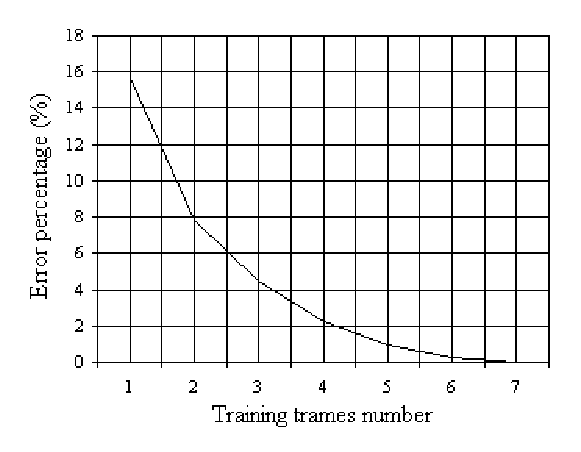
\includegraphics[width=2.7in]{Figure3}
      % where an .eps filename suffix will be assumed under latex, 
      % and a .pdf suffix will be assumed for pdflatex
      \label{fig:fig2b}}}
  \caption{Optimal number of frames in the training data set.}
  \label{fig:fig2}
\end{figure}

% For this to work you need to (in preamble.tex):
% - remove \usepackage{subfig}
% - add \usepackage{caption}
% - add \usepackage{subcaption}
% \begin{figure}
%   \centering
%   \begin{subfigure}[b]{0.3\textwidth}
%     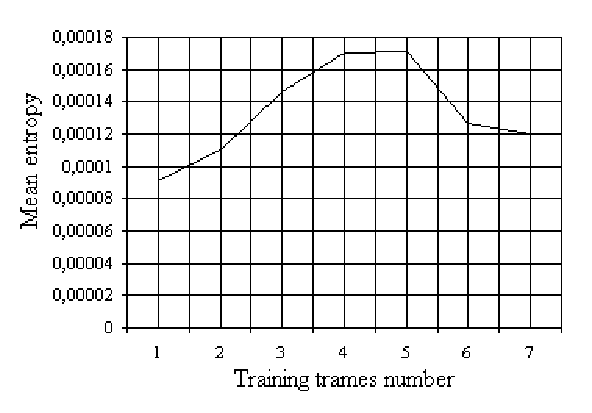
\includegraphics[width=\textwidth]{Figure2}
%     \caption{Mean Entropy.}
%     \label{fig:fig3a}
%   \end{subfigure}%
%   ~ %add desired spacing between images, e. g. ~, \quad, \qquad etc.
%   % (or a blank line to force the subfigure onto a new line)
%   \begin{subfigure}[b]{0.3\textwidth}
%     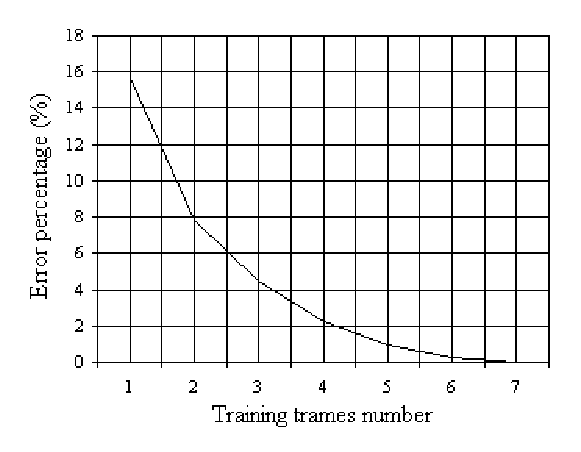
\includegraphics[width=\textwidth]{Figure3}
%     \caption{Error Percentage.}
%     \label{fig:fig3b}
%   \end{subfigure}
%   \caption{Optimal trames number in the training data set.}
%   \label{fig:fig3}
% \end{figure}

Incluso podemos poner una tabla ``apaisada'', como en la
\ref{tablas2006}, donde se muestra un resumen de los resultados
obtenidos en una serie de experimentos de localizaci�n de locutores.

\clearpage
% \begin{table}[H]\centering
\begin{sidewaystable}[hbtp]
  \begin{center}

    \begin{tabular}{||l|c|c|c|c|c||}
      \hline \hline
      & UKA & ITC & AIT & UPC & IBM\\
      \hline
      \hline
      Pcor & $57.0\pm1.4\%$ & $84.0\pm3.3\%$ & $47.0\pm3.1\%$ & $20.0\pm2.5\%$ & $67.0\pm2.9\%$ \\
      \hline
      Bias fine (x:y:z) [mm] & $20:-42:-75$ & $45:27:-41$ & $-27:-77:-40$ & $-59:112:52$ & $91:-69:-38$ \\
      \hline
      Bias fine+gross (x,y,z) [mm] & $735:-93:-258$ & $67:439:-134$ & $17:-402:-118$ & $-141:255:39$ & $474:-141:-14$ \\
      \hline
      AEE fine [mm] = MOTP & $210$ & $130$ & $266$ & $344$ & $228$ \\
      \hline
      Fine+gross [mm] & $1201$ & $632$ & $1006$ & $1188$ & $884$ \\
      \hline
      Loc. frames & $5035$ & $22$ & $995$ & $977$ & $1023$ \\
      \hline
      Ref. duration (s) & $6287.0$ & $596.0$ & $1143.0$ & $1180.0$ & $1194.0$ \\
      \hline \hline
    \end{tabular}
    \caption{Resultados TEST CLEAR 2006.}
    \label{tablas2006}
  \end{center}
\end{sidewaystable}
% \end{table}


\section{Conclusiones}
\label{sec:conclusiones-resultados}

Blah, blah, blah.


%%% Local Variables:
%%% TeX-master: "../book"
%%% End:
